\documentclass{beamer}
\usetheme{Warsaw}
\usecolortheme{beaver}
\title[Bias, Variance and Parsimony in Regression Analysis]{Bias, Variance and Parsimony in Regression Analysis\\ECS 256 Winter 2014}
\author[Norm Matloff]{
Christopher Patton, \texttt{cjpatton@ucdavis.edu}\\
Alex Rumbaugh, \texttt{aprumbaugh@ucdavis.edu}\\
Thomas Provan,\texttt{tcprovan@ucdavis.edu}\\
Olga Prilepova, \texttt{prilepova@gmail.com}\\
John Chen, \texttt{jhochen@ucdavis.edu}}
\institute{ECS 256, Winter 2014\\ \Large{UC Davis}}
\date{March 12, 2014}
\begin{document}

\begin{frame}
\titlepage
\end{frame}


\begin{frame}{Introduction}
%This is the introduction.
\end{frame}

% Alex's Section -----------------------------------------------------------------
\author[Alex Rumbaugh]{C. Patton, A. Rumbaugh, T. Provan, O. Prilepova, J. Chen}
\begin{frame}
    \frametitle{California Housing Data}
	\begin{itemize}
		\item { }
		\item {Derived from 1990 Census}
		\item {Response Variable: median house value}
		\item {Predictor Variables: median income, housing median age, total rooms, total bedrooms, population, households, latitude, and longitude}
	\end{itemize}
\end{frame}

\begin{frame}
    \frametitle{Parsimony}
	\begin{tabular}{ | c | p{3cm} | p{3cm} | c  |}
\hline
Method&Parsimony (k=0.01) & Parsimony (k=0.05) & Significance Testing \\
\hline
Columns\newline Deleted& Total Rooms \newline Total Bedrooms & Total Rooms \newline Total Bedrooms \newline Median Age & None \\
\hline
Adjusted RSquared & 0.6321316 & 0.6218261 & 0.6369649 \\
\hline
\end{tabular}
\end{frame}

\begin{frame}[fragile]
    \frametitle{Regression Coefficients}
\begin{verbatim}
Coefficients:
                 Estimate Std. Error t value Pr(>|t|)    
(Intercept)    -3.594e+06  6.254e+04 -57.468  < 2e-16 ***
Median.Income   4.025e+04  3.351e+02 120.123  < 2e-16 ***
Median.Age      1.156e+03  4.317e+01  26.787  < 2e-16 ***
Total.Rooms    -8.182e+00  7.881e-01 -10.381  < 2e-16 ***
Total.Bedrooms  1.134e+02  6.902e+00  16.432  < 2e-16 ***
Population     -3.854e+01  1.079e+00 -35.716  < 2e-16 ***
Households      4.831e+01  7.515e+00   6.429 1.32e-10 ***
Latitude       -4.258e+04  6.733e+02 -63.240  < 2e-16 ***
Longitude      -4.282e+04  7.130e+02 -60.061  < 2e-16 ***
\end{verbatim}
\end{frame}

\begin{frame}[fragile]
    \frametitle{Latitude \& Longitude}
\begin{verbatim}
	Latitude       -4.258e+04  6.733e+02 -63.240  < 2e-16 ***
	Longitude      -4.282e+04  7.130e+02 -60.061  < 2e-16 ***
\end{verbatim}
\begin{itemize}
\item "Center of Gravity"
\item Avoid Overfitting
\end{itemize}
	
\end{frame}

\begin{frame}[fragile]
    \frametitle{Understanding}
	\begin{verbatim}
Coefficients:
                Estimate Std. Error t value Pr(>|t|)    
(Intercept)   -32165.268   2167.358  -14.84   <2e-16 ***
Median.Income  43094.918    284.263  151.60   <2e-16 ***
Median.Age      2000.544     45.080   44.38   <2e-16 ***
Population       -43.045      1.127  -38.20   <2e-16 ***
Households       152.700      3.344   45.66   <2e-16 ***
\end{verbatim}
\end{frame}

\begin{frame}
	\begin{figure}
 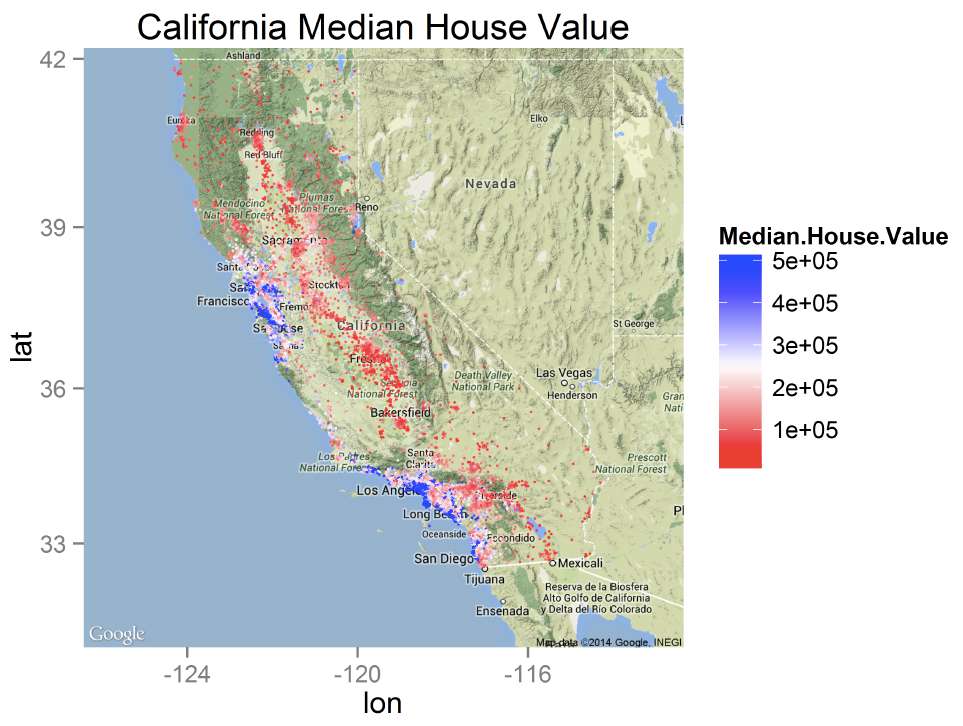
\includegraphics[scale=0.3]{figures/california.png}
\end{figure}
\end{frame}

\begin{frame}
	\begin{figure}
 \includegraphics[scale=0.3]{figures/losangeles.png}
\end{figure}
\end{frame}

\begin{frame}
	\begin{figure}
 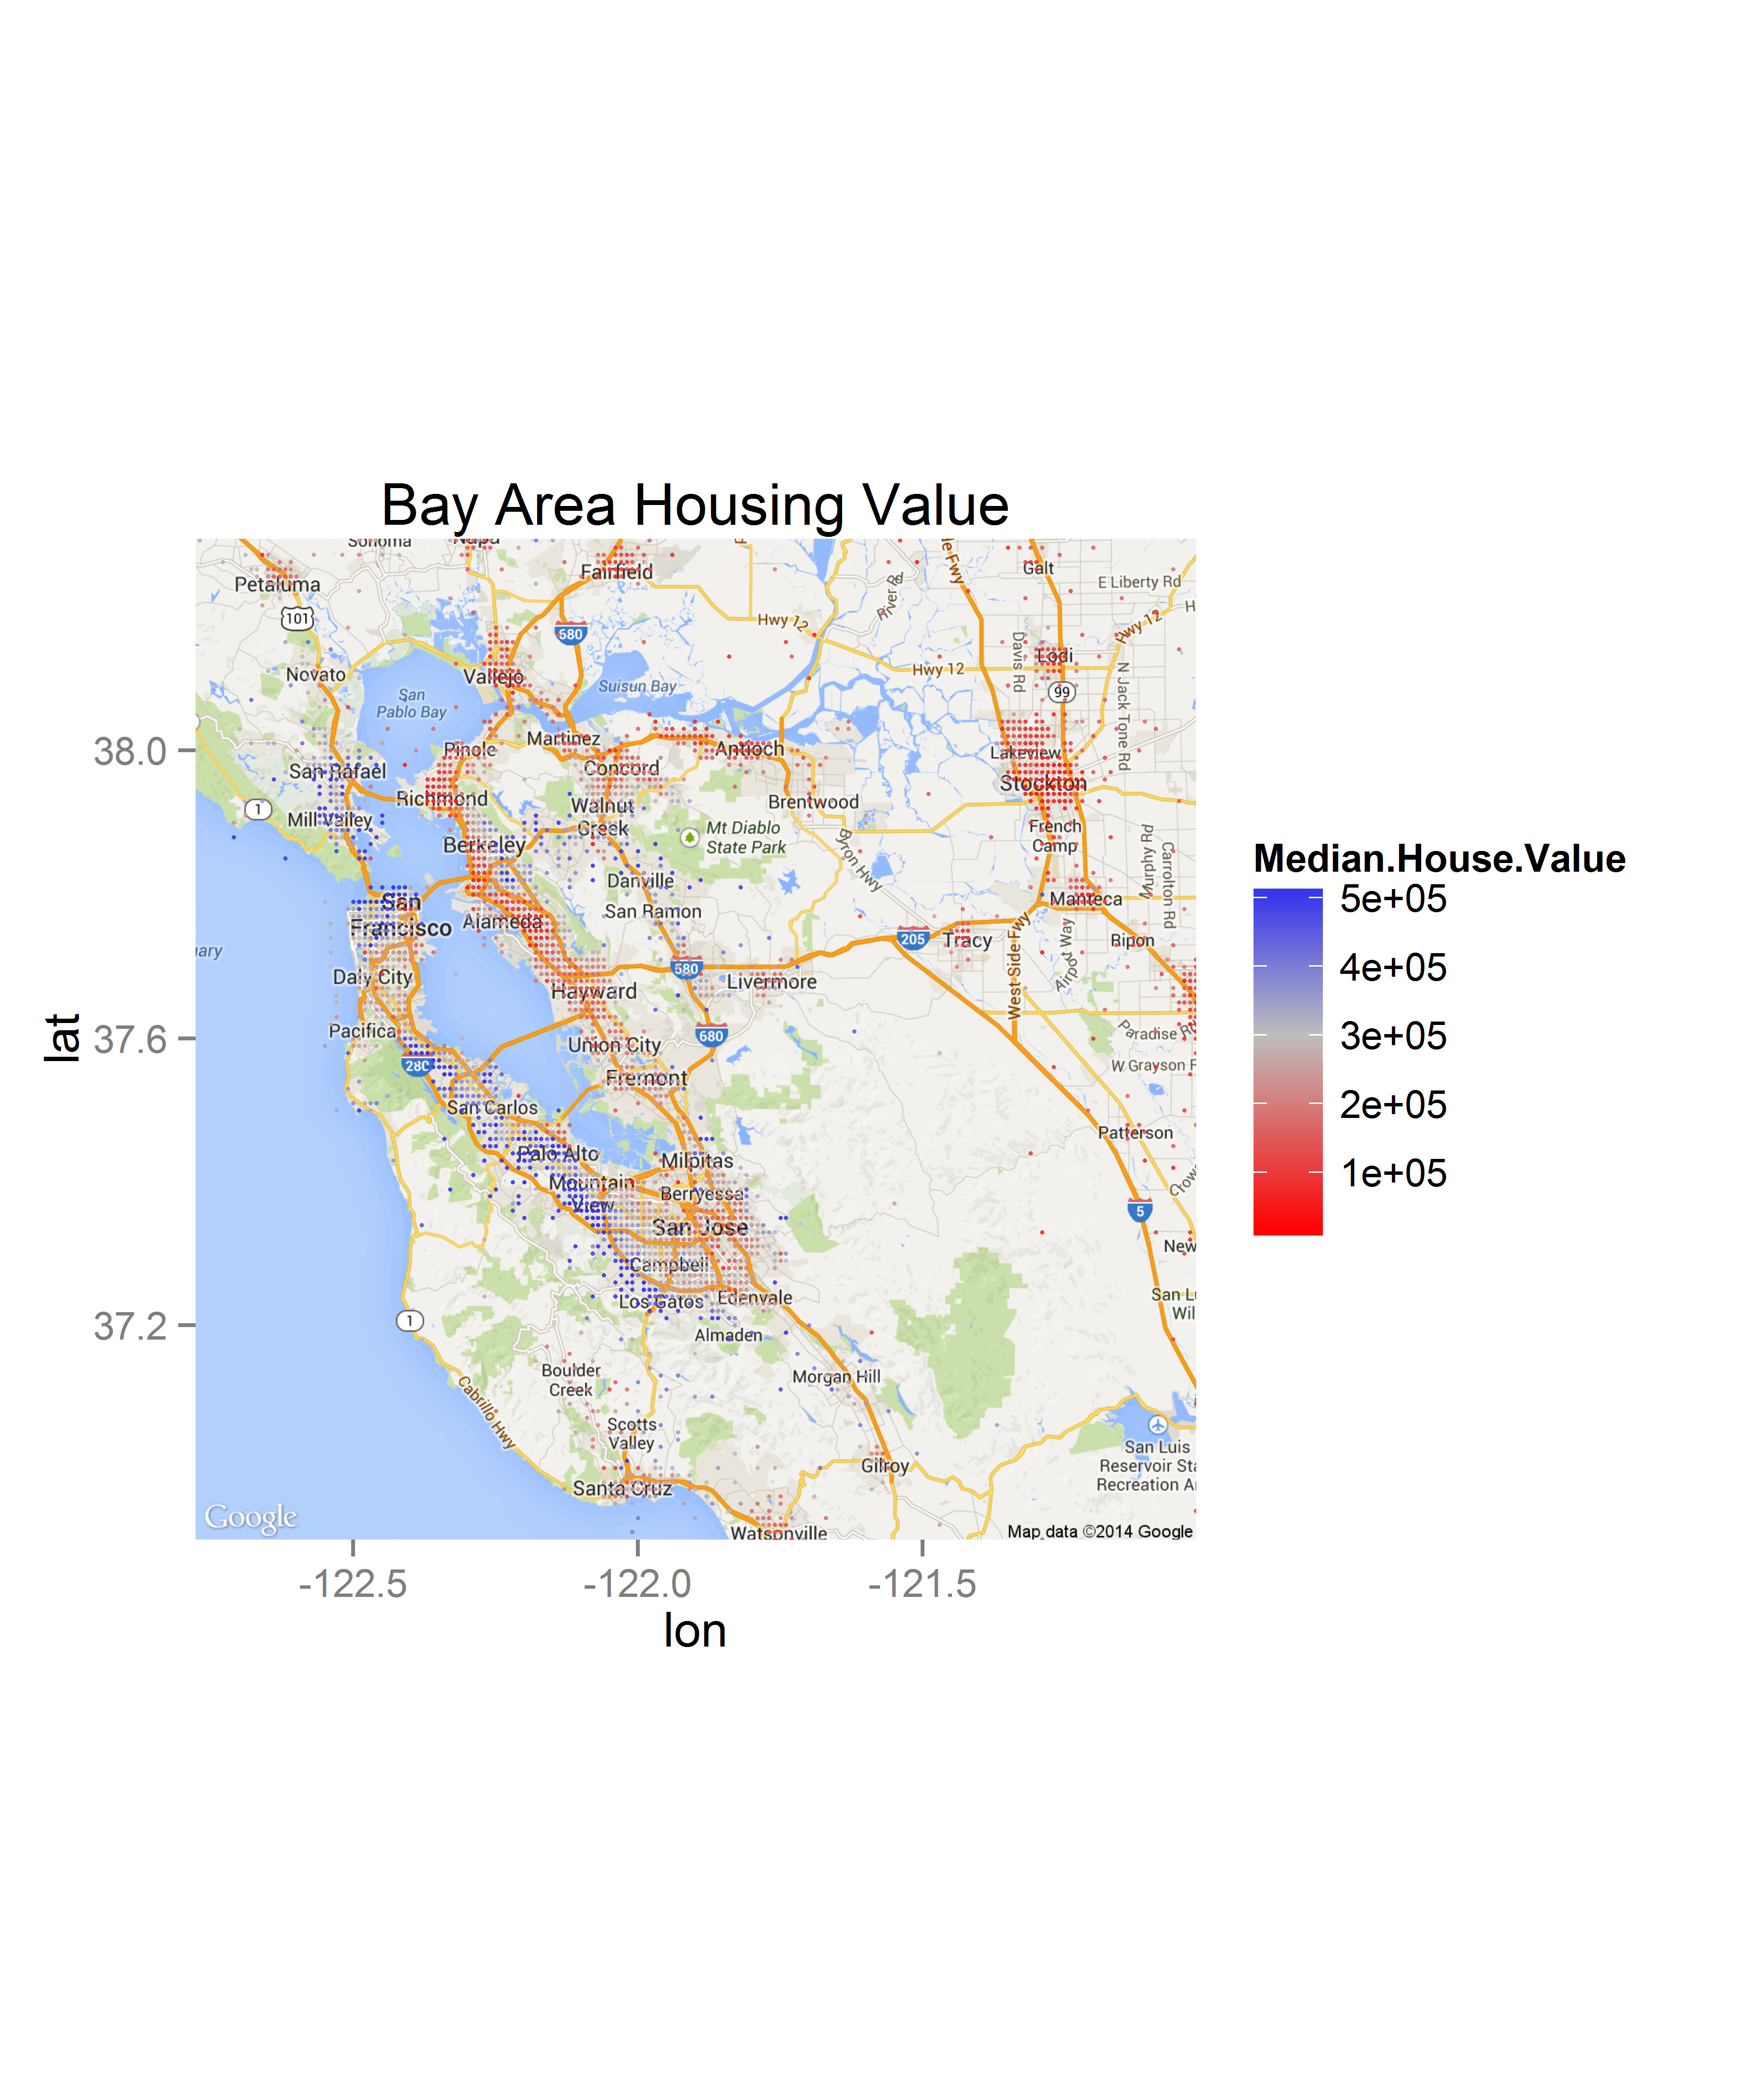
\includegraphics[scale=0.3]{figures/bayarea.png}
\end{figure}
\end{frame}

% End Alex's Section--------------------------------------------------------------

% Olga's Section--------------------------------------------------------------
\author[Olga Prilepova]{C. Patton, A. Rumbaugh, T. Provan, O. Prilepova, J. Chen}

\begin{frame}
\frametitle{Census Based on 1994}
\end{frame}

\begin{frame}
\frametitle{Age}
\end{frame}

\begin{frame}
\frametitle{}

\begin{figure}
 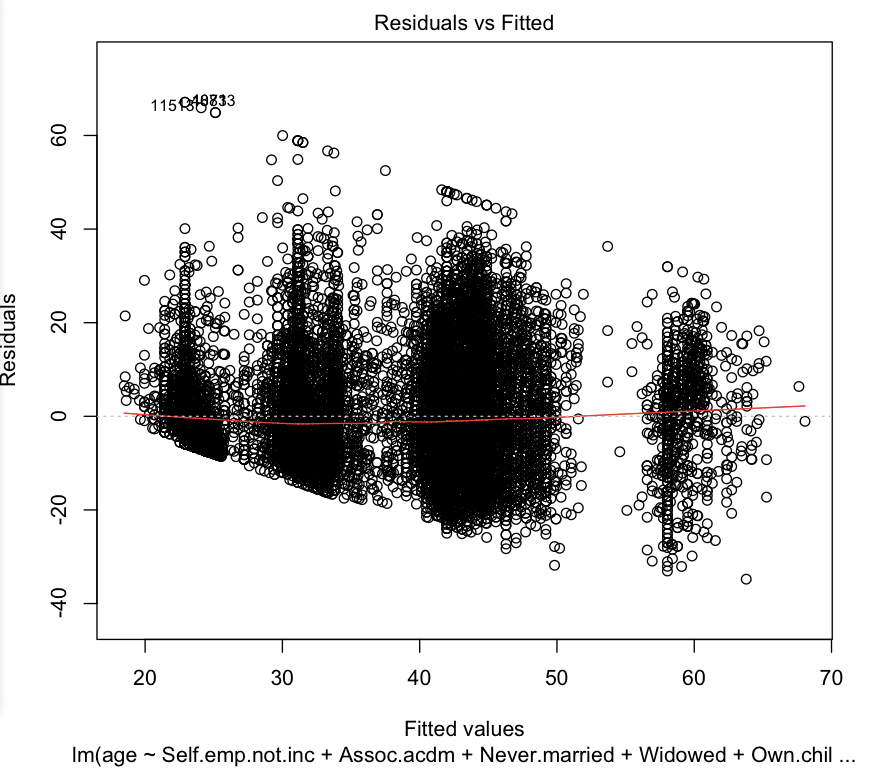
\includegraphics[scale=0.3]{figures/ageResidCensus.png}
 \label{fig:ageResidCensus}
\end{figure}
 
\end{frame}

\begin{frame}
\frametitle{Census Based on 1994}
% Census Sex Coefficients
\end{frame}

\begin{frame}
\frametitle{Census Based on 1994}
% Census Salary Coefficients
\end{frame}

\begin{frame}
%Picture of predicted vs actual age
\begin{figure}
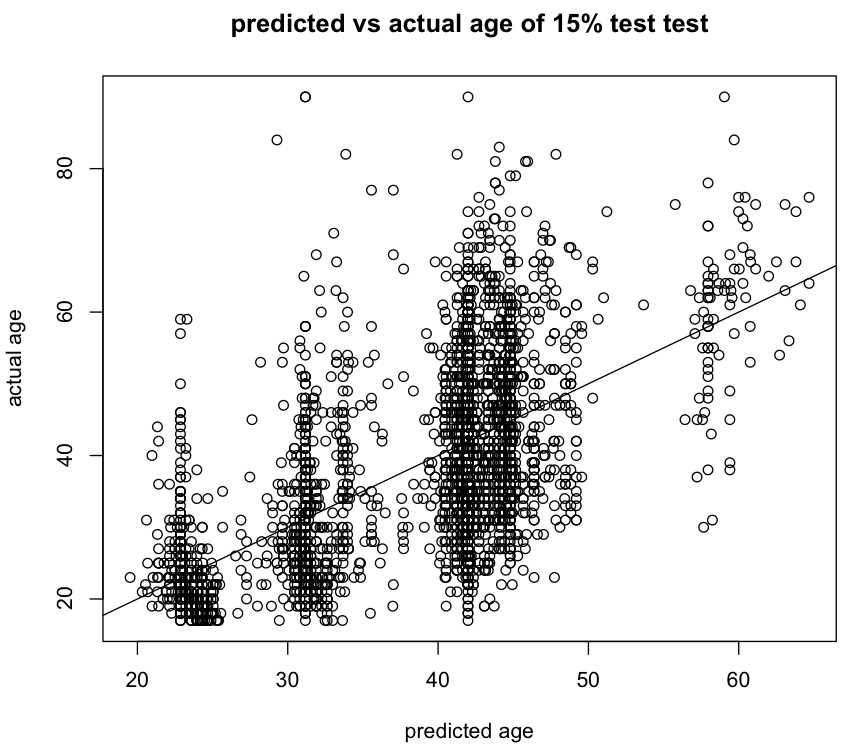
\includegraphics[scale=0.3]{figures/predVsActualCensus.png}
\label{fig:predVsActualCensus}
\end{figure}
\end{frame}

\begin{frame}
%Picture of predicted vs actual age

\begin{figure}
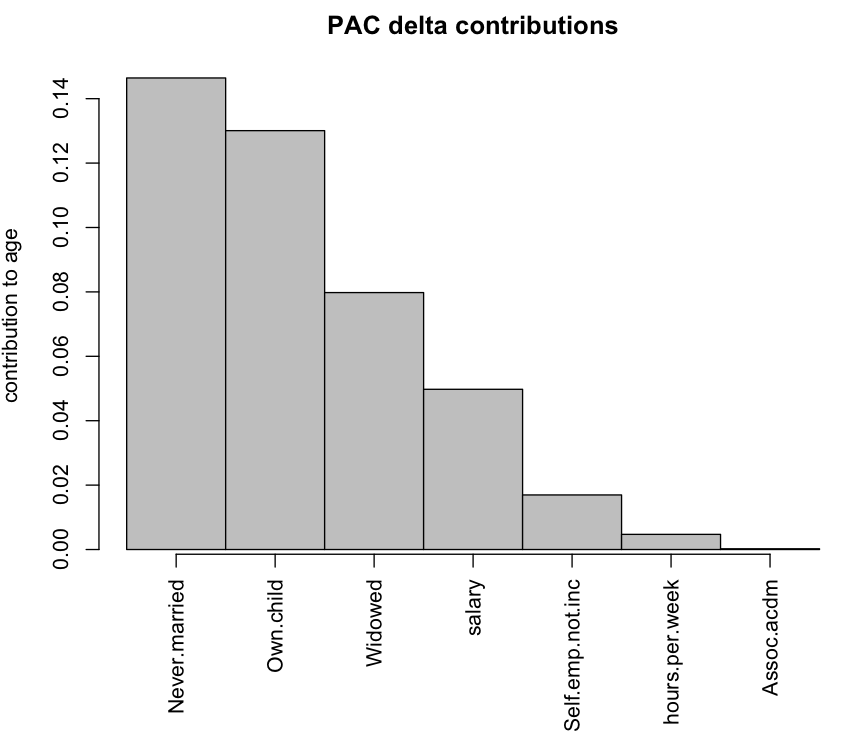
\includegraphics[scale=0.3]{figures/ageContrib.png}
\caption{}
 \label{fig:ageContrib}
\end{figure}

\end{frame}
% End Olga's Section--------------------------------------------------------------

% Begin Chris' Section--------------------------------------------------------------
\author[Christopher Patton]{C. Patton, A. Rumbaugh, T. Provan, O. Prilepova, J. Chen}

\begin{frame}
\frametitle{}
%Slide 1
\end{frame}

\begin{frame}
\frametitle{}
%Slide 2
\end{frame}

\begin{frame}
\frametitle{}
%Slide 3
\end{frame}

\begin{frame}
\frametitle{}
%Slide 4
\end{frame}

\begin{frame}
\frametitle{}
%Slide 5
\end{frame}

% End Chris' Section--------------------------------------------------------------
% Thomas' Section--------------------------------------------------------------

% Theme: Problem 2b Parsimony on Simulated Data
\author[Thomas Provan]{C. Patton, A. Rumbaugh, T. Provan, O. Prilepova, J. Chen}

\begin{frame}
\frametitle{Testing Parsimony on Simulated Data}
%Slide 1
\end{frame}

\begin{frame}
\frametitle{Testing Parsimony on Simulated Data}
%Slide 2

\begin{tabular}{| l  r | c | c | c |}

\hline

	&&	prsm(k=0.01)&	prsm(k=0.05)&	sig test	\\
\hline

n=100&	Run 1&	$X_1 ,X_2, X_3, X_9$&	$X_1, X_2, X_3$&		$X_1, X_2, X_3$	\\
	&	Run 2&	$X_1, X_2, X_3$&		$X_1, X_2, X_3$&		$X_1, X_2, X_3$	\\
	&	Run 3&	$X_1, X_2, X_3$&		$X_1, X_2, X_3$&		$X_1, X_2, X_3$	\\

\hline

n=1000&	Run 1&	$X_1, X_2, X_3$&		$X_1, X_2, X_3$&		$X_1, X_2, X_3, X_4$	\\
	&	Run 2&	$X_1, X_2, X_3$&		$X_1, X_2, X_3$&		$X_1, X_2, X_3$		\\
	&	Run 3&	$X_1, X_2, X_3$&		$X_1, X_2, X_3$&		$X_1, X_2, X_3$		\\
	
\hline
			
n=10K&	Run 1&	$X_1, X_2, X_3$&		$X_1, X_2, X_3$&		$X_1, X_2, X_3, X_4$		\\
	&	Run 2&	$X_1, X_2, X_3$&		$X_1, X_2, X_3$&		$X_1, X_2, X_3, X_4$		\\
	&	Run 3&	$X_1, X_2, X_3$&		$X_1, X_2, X_3$&		$X_1, X_2, X_3, X_4, X_9$		\\

\hline
			
n=100K&	Run 1&	$X_1, X_2, X_3$&		$X_1, X_2, X_3$&		$X_1, X_2, X_3, X_4$		\\
	&	Run 2&	$X_1, X_2, X_3$&		$X_1, X_2, X_3$&		$X_1, X_2, X_3, X_4, X_9$		\\
	&	Run 3&	$X_1, X_2, X_3$&		$X_1, X_2, X_3$&		$X_1, X_2, X_3, X_4, X_9$		\\

\hline

\end{tabular}


\end{frame}

\begin{frame}
\frametitle{Testing Parsimony on Simulated Data}

\begin{tabular}{| l | c | c | c | c | c | c | c | c | c | c |}



\hline
\textbf{prsm(k=0.01)}&	$X_1$&	$X_2$&	$X_3$&	$X_4$&	$X_5$&	$X_6$&	$X_7$&	$X_8$&	$X_9$&	$X_{10}$\\
\hline
N = 100&			1&	1&	1&	0.24&	0.11&	0.14&	0.21&	0.22&	0.26&	0.28 	\\
N = 1000&			1&	1&	1&	0.08&	0&	0&	0&	0&	0&	0	\\
N = 10000&			1&	1&	1&	0&	0&	0&	0&	0&	0&	0	\\
N = 100000&		1&	1&	1&	0&	0&	0&	0&	0&	0&	0	\\
N = 1M&			1&	1&	1&	0&	0&	0&	0&	0&	0&	0	\\
\hline		

\\
								
									\\		
\hline					
\textbf{prsm(k=0.05)}&	$X_1$&	$X_2$&	$X_3$&	$X_4$&	$X_5$&	$X_6$&	$X_7$&	$X_8$&	$X_9$&	$X_{10}$\\
\hline
N = 100&			1&	1&	0.99&	0.1&	0.02&	0.05&	0.04&	0.03&	0.07&	0.02	\\
N = 1000&			1&	1&	1&	0&	0&	0&	0&	0&	0&	0	\\
N = 10000&			1&	1&	1&	0&	0&	0&	0&	0&	0&	0	\\
N = 100000&		1&	1&	1&	0&	0&	0&	0&	0&	0&	0	\\
N = 1M&			1&	1&	1&	0&	0&	0&	0&	0&	0&	0	\\
\hline
\\

								
											\\
\hline
\textbf{Sig Test}&	$X_1$&	$X_2$&	$X_3$&	$X_4$&	$X_5$&	$X_6$&	$X_7$&	$X_8$&	$X_9$&	$X_{10}$\\
\hline
N = 100&		1&	1&	1&	0.14&	0.03&	0.05&	0.05&	0.03&	0.09&	0.04	\\
N = 1000&		1&	1&	1&	0.31&	0.02&	0.05&	0.05&	0.05&	0.02&	0.04	\\
N = 10000&		1&	1&	1&	1&	0.04&	0.01&	0.07&	0.07&	0.03&	0.06	\\
N = 100000&	1&	1&	1&	1&	0.35&	0.06&	0.09&	0.03&	0.05&	0.03	\\
N = 1M&		1&	1&	1&	1&	1&	0.05&	0.03&	0.08&	0.02&	0.03	\\
\hline
\end{tabular}


\end{frame}

\begin{frame}
\frametitle{Testing Parsimony on Simulated Data}
%Slide 4
\end{frame}

\begin{frame}
\frametitle{Maybe something else?}
%Slide 5
\end{frame}
% End Thomas' Section--------------------------------------------------------------
% John's Section--------------------------------------------------------------

\author[John Chen]{C. Patton, A. Rumbaugh, T. Provan, O. Prilepova, J. Chen}
% Theme: Automobile Analysis & Accurate Predictors
\begin{frame}
\frametitle{Small N, Large P}
%Slide 1
\end{frame}

\begin{frame}
\frametitle{}
%Slide 2
\end{frame}

\begin{frame}
\frametitle{}
%Slide 3
\end{frame}

\begin{frame}
\frametitle{}
%Slide 4
\end{frame}

\begin{frame}
\frametitle{}
%Slide 5
\end{frame}
% End John's Section--------------------------------------------------------------
\end{document}